\paragraph{QuizziPedia::Back-End::App::Models::TopicModel}
\label{QuizziPedia::Back-End::App::Models::topicModel}
\begin{figure}
	\centering
	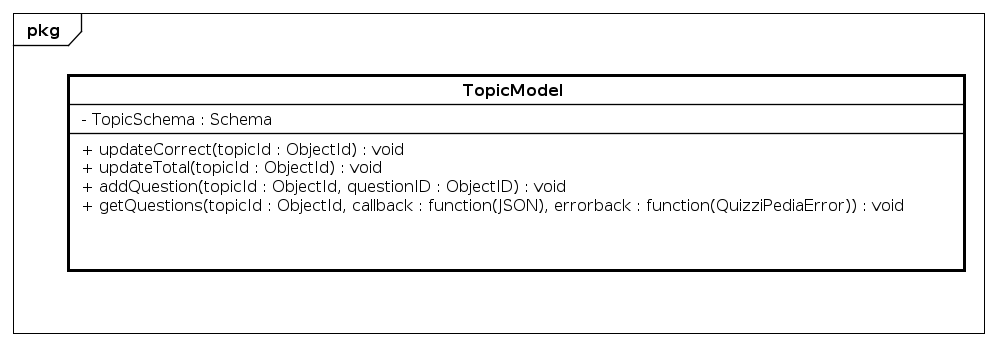
\includegraphics[scale=0.45]{UML/Package/QuizziPedia_Back-End_App_Models_topicModel.png}
	\caption{QuizziPedia::Back-End::App::Models::topicModel}
\end{figure}
\begin{itemize}
	\item \textbf{Descrizione} \\
	Classe che modella gli argomenti all'interno dell'applicazione.
	\item \textbf{Utilizzo} \\
	Viene utilizzata per rappresentare i dati relativi agli argomenti all'interno dell'applicazione. Si interfaccia con la libreria \textit{Mongoose\ped{G}} per la creazione dello schema e dei relativi metodi statici o di istanza.
	\item \textbf{Relazioni con altre classi}
		\begin{itemize}
			\item 
		\end{itemize}
	\item \textbf{Attributi}
		\begin{itemize}
			\item \textbf{- topicSchema: Schema} \\
			Questo campo dati rappresenta lo schema Mongoose degli argomenti di QuizziPedia. Lo schema prevede i seguenti attributi:
				\begin{itemize}
					\item \texttt{name} di tipo \texttt{String}, rappresenta il nome dell'argomento;
					\item \texttt{level} di tipo \texttt{Number}, rappresenta il livello medio degli utenti che hanno svolto almeno un allenamento dell'argomento;
					\item \texttt{correctAnswers} di tipo \texttt{Number}, rappresenta il numero totale di domande che gli utenti hanno risposto correttamente durante un allenamento dell'argomento; 
					\item \texttt{totalAnswers} di tipo \texttt{Number}, rappresenta il numero totale di domande che gli utenti hanno risposto durante un allenamento dell'argomento;
					\item \texttt{question} di tipo \texttt{Array}, contiene oggetti di tipo \texttt{Question} che rappresentano i riferimenti agli identificativi nel database delle domande appartenenti all'argomento.
				\end{itemize}
		\end{itemize}
	\item \textbf{Metodi}
		\begin{itemize}
			\item 
		\end{itemize}
\end{itemize}